\enteteThematiqueObligatoire{}
\enteteCorrection{}

%%%%%%%%%%%%%%%%%%%%%%%%%%%%%%%%%%%%%%%%%%%%%%%%%%%%%%%%%%%%%%%%%%%%%%%%%%
\encadreTDExo{1 - Conversion de signaux courants}{
\begin{itemize}[label=$\triangleright$,leftmargin=*]
	\item rappel des fréquences mises en jeu dans les signaux habituels
\end{itemize}
}

%%%%%%%%%%%%%%%%%%%%%%%%%%%%%%%%%%%%
\subsection*{Signal audio}

\begin{enumerate}
	\item Rappeler l'intervalle de fréquences des signaux audibles par l'être humain.
	
\answer{Entre $20\operatorname{Hz}$ et $20\operatorname{kHz}$.}	

	\item Quelle est la fréquence minimale pour échantillonner correctement un signal audio ?
	
\answer{Afin de respecter le critère de Nyquist-Shannon, à savoir qu'il faut au moins échantillonner 2 points par période d'un signal pour pouvoir le reconstituer fidèlement, il faut une fréquence d'échantillonnage supérieure à $40\operatorname{kHz}$.}

Les signaux audio "classiques" (CD audio par exemple) sont échantillonnés à une fréquence $F_{Eclassique} = 44.1\operatorname{kHz}$ et chaque échantillon est codé sur 16~bits. 

Les signaux HRA (Audio Haute Résolution) sont échantillonnés à une fréquence $F_{EHRA1} = 96\operatorname{kHz}$ ou $F_{EHRA2} = 192\operatorname{kHz}$ et chaque échantillon est codé sur 24~bits.

	\item Ces fréquences sont-elles bien choisies ?

\answer{Elles respectent toutes le critère de Nyquist-Shannon, puisque $F_E > 40\operatorname{kHz}$.}

	\item Combien de niveau logique différent y a-t-il pour chacune de ces normes ?

\answer{Pour la version "classique", on a $2^{16}$ niveaux logiques différents (soit 65536 niveaux).

Pour la version HRA, on a $2^{24}$ niveaux logiques différents (soit plus de 16 millions de niveaux).}

	\item Quelle quantité d'espace numérique (en octets) faut-il prévoir pour stocker une heure de données sonores :
	\begin{enumerate}
		\item au format "classique", stéréo ?

\answer{En stéréo, il y a 2 voies. On les échantillonne chacune à 44100~Hz, soit 44100 échantillons par seconde de 16 bits chacun. 

La quantité de données est alors de : 
$$DATA = 2(voies) \cdot 16(bits) \cdot 44100(ech/s) \cdot 3600(s) / 8(bits) = 635.04\operatorname{Mo}$$
}		
		
		\item au format HRA-192, en 5.1 ?
\answer{En 5.1, il y a 6 voies. On les échantillonne chacune à 192000~Hz, soit 192000 échantillons par seconde de 24 bits chacun. 

La quantité de données est alors de : 
$$DATA = 6(voies) \cdot 24(bits) \cdot 192000(ech/s) \cdot 3600(s) / 8(bits) = 12.5\operatorname{Go}$$
}
	\end{enumerate}
	
\end{enumerate}

%%%%%%%%%%%%%%%%%%%%%%%%%%%%%%%%%%%%
\subsection*{Signal vidéo}

On s'intéresse au capteur \textbf{CMV50000} de la société \textit{CMOSIS}, capteur 8K@30fps - au prix d'environ 3500\$ (juin 2018) dont la documentation est donnée en annexe.

\seance{On peut rappeler le principe d'un capteur CMOS = ensemble de photodiodes et leur système d'amplification. Le tout est lié à plusieurs convertisseurs analogique/numérique en parallèle.}

\begin{enumerate}
	\item Quelle est la taille de l'image de ce capteur ? Combien cela fait-il de pixels ?
\answer{
	On peut lire dans la documentation : 7920 (H) x 6004 (V) soit un total de 47.5 millions de pixels.
}
	\item Combien de convertisseurs analogique-numérique embarquent ce capteur ? 
	Quelle est la résolution des ADC ?
\answer{
	Le constructeur annonce : \textbf{22 LVDS at 830 Mbps} comme sortie. Cela correspond à \textbf{22 convertisseurs} placés en parallèle.
	
	On trouve également que le nombre d'électrons récupérés en sortie en \textbf{pleine échelle} (Full well charge) est de 14500 e-. On a également le taux de conversion de 0.272 DN/e. On a alors que la pleine échelle est d'environ 3950 DN. 
	Cela correspond bien aux 12 bits annoncés par le constructeur.	
}

\seance{On peut rappeler ici que les capteurs CMOS sont des matrices de photodiodes qui transforment un flux lumineux en électrons.}

	\item La vitesse de transfert donnée est-elle suffisante pour prendre des images en 8K (7680 x 4320 pixels) à 30 images/seconde ?
	
\answer{
	Pour une image en 8K, soit 7680 x 4320 pixels, chacun codé sur 12 bits, à 30 images/seconde, cela donne : 
	
	$$DATA = 7680 \cdot 4320 \cdot 12(bits) \cdot 30(fps) = 11.94\operatorname{Gbps} = 1.5\operatorname{Gops}$$
	
	Comme il y a 22 sorties en parallèle, chacune produit donc un flux de donnée de : $DATA_{LVDS} = DATA / 22 = 543\operatorname{Mbps} = 68\operatorname{Mops}$.
}
\end{enumerate}

%%%%%%%%%%%%%%%%%%%%%%%%%%%%%%%%%%%%%%%%%%%%%%%%%%%%%%%%%%%%%%%%%%%%%%%%%%
\encadreTDExo{2 - Système numérique}{
\begin{itemize}[label=$\triangleright$,leftmargin=*]
	\item étude d'un signal échantillonné
	\item critère de Shannon-Nyquist
\end{itemize}
}

Que peut-on dire des signaux suivants ?

\begin{figure}[!h]
	\centering
	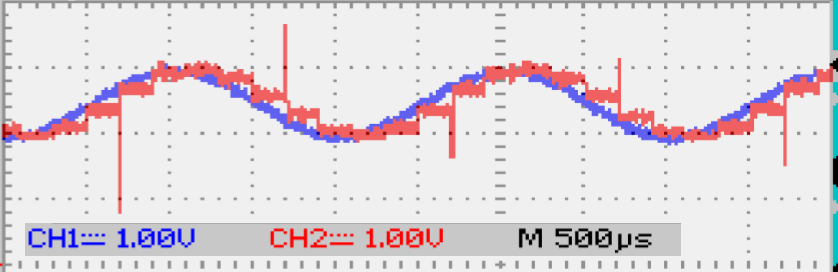
\includegraphics{images/TD/signal_num_1.png}
	\caption{Sortie d'un filtre numérique}
\end{figure}


\answer{
Cette figure correspond à la réponse d'un système numérique qui échantillonne à une fréquence de 5 kHz (ou une période de 200 $\mu{}$s - largeur d'un palier).
}

\begin{figure}[!h]
	\centering
	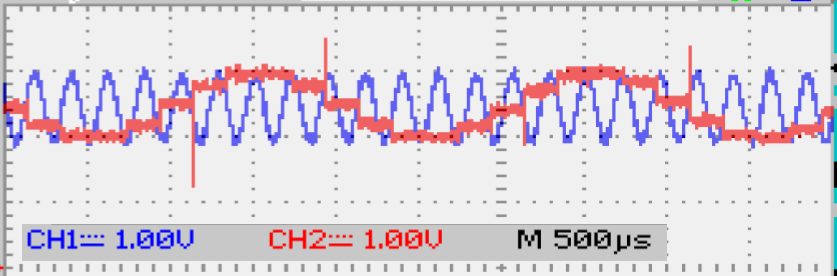
\includegraphics{images/TD/signal_num_2.png}
	\caption{Sortie d'un filtre numérique}
\end{figure}

\answer{
Cette figure correspond à la réponse du même système numérique que précédemment.

On remarque ici que le signal de sortie n'a pas la même fréquence de le signal de départ. Le système n'est donc pas linéaire !! On assiste ici à un repliement de spectre dû à l'échantillonnage.
}

\seance{On peut ici dessiner le spectre du signal initial, et de la version échantillonné de ce signal pour montrer le repliement.}

%%%%%%%%%%%%%%%%%%%%%%%%%%%%%%%%%%%%%%%%%%%%%%%%%%%%%%%%%%%%%%%%%%%%%%%%%%
\encadreTDExo{3 - Entrées/Sorties Numériques}{
\begin{itemize}[label=$\triangleright$,leftmargin=*]
	\item étude de la documentation technique d'un CAN
	\item entrée/sortie série/parallèle
\end{itemize}
}


On s'intéresse à présent à 2 convertisseurs analogiques-numériques différents, dont une partie des documentations techniques sont données en annexe :
\begin{itemize}
	\item \textbf{TLC548} de \textit{Texas Instruments} (environ 3\$ - juin 2018)
	\item \textbf{AD9230} de \textit{Analog Devices} (environ 80\$ - juin 2018)
\end{itemize}

\begin{enumerate}
	\item A partir de ces deux documentations, remplir le tableau suivant :

\begin{tabular}{|c|p{3cm}|p{3cm}|}
\hline 
 & TLC548 & AD9230 \\ 
\hline 
Type de sortie &  &  \\ 
\hline 
$F_{Emax}$ &  &  \\ 
\hline 
Résolution &  &  \\ 
\hline 
Alimentation &  &  \\ 
\hline 
\end{tabular} 
	
\answer{
\begin{tabular}{|c|p{3cm}|p{3cm}|}
\hline 
 & TLC548 & AD9230 \\ 
\hline 
Type de sortie & Série\footnote{Liaison type SPI avec les signaux : CS-IO\_CLOCK-DATA\_OUT} & Parallèle - LVDS\footnote{\textit{Low Voltage Differential Signaling} - nouvelle norme pour la transmission de signaux électriques à haute fréquence - plusieurs centaines de MHz - sur une ligne symétrique / signal différentiel} \\ 
\hline 
$F_{Emax}$ & 45.5~ksps & 250~Msps \\ 
\hline 
Résolution & 8~bits & 12~bits \\ 
\hline 
Alimentation & 3~à~6~V & 1.8~V \\ 
\hline 
\end{tabular} 
}	
	
	\item A l'aide de la documentation technique du \textbf{TLC548}, 
	\begin{enumerate}
		\item Expliquer à quoi correspondent les différents éléments du \textbf{diagramme fonctionnel} donnée en page 2.

\answer{
	\begin{center}
		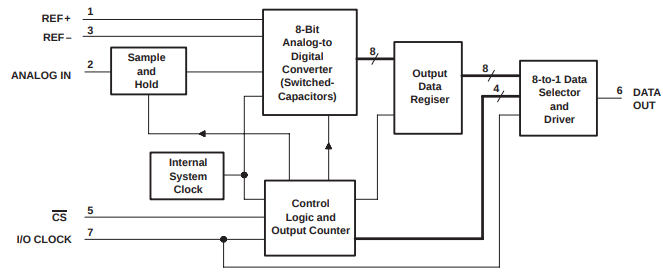
\includegraphics{images/TD/TLC548_bloc.png}
	\end{center}

	\begin{itemize}
		\item[$\bullet$] \textbf{8-Bit Analog-to-Digital Converter} : convertisseur avec :
		\begin{itemize}
			\item[$\Box$] 2 entrées de référence REF+ et REF-
			\item[$\Box$] 1 entrée pour le signal analogique à convertir
			\item[$\Box$] 1 sortie sur 8 bits pour la donnée numérique
			\item[$\Box$] des entrées de contrôle
		\end{itemize}
		\item[$\bullet$] \textbf{Data Output Register} : bloc permettant de mémoriser la donnée le temps d'une autre conversion
		\item[$\bullet$] \textbf{8-to-1 Data Selector and Driver} : bloc permettant de transformer la donnée numérique parallèle en donnée numérique série, à partir de l'horloge d'entrée
		\item[$\bullet$] \textbf{Sample and Hold} : échantillonneur bloqueur permettant d'avoir un signal analogique stable durant tout le temps de la conversion\footnote{On peut prendre un peu de temps pour montrer le fonctionnement via le schéma proposé dans la documenation technique}
		\item[$\bullet$] \textbf{Control Logic and Output Counter} : bloc de contrôle de la séquence de conversion
	\end{itemize}
}		

		\item Expliquer l'opération de conversion et de récupération des données à partir de la \textbf{séquence} donnée en page 3.

\answer{
	\begin{center}
		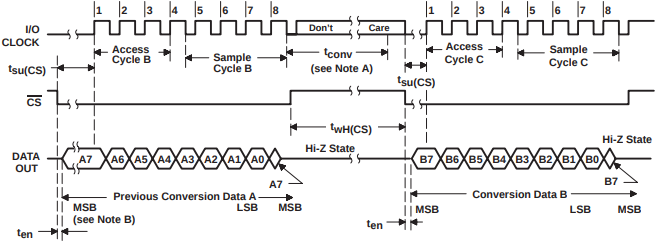
\includegraphics{images/TD/TLC548_sequence.png}
	\end{center}
	
	La conversion se fait lorsque le signal $CS$ passe à '1'. La conversion dure jusqu'à $t_{conv} = 17\operatorname{\mu{}s}$ (d'après la documentation technique). 
	
	La donnée est ensuite prête dans le registre de données. Il faut forcer le signal $CS$ à '0' pour débuter la discussion avec le composant.
	Il faut appliquer un signal d'horloge (jusqu'à $2.048\operatorname{MHz}$ d'après la documentation technique).
}
		\item Combien de temps faut-il entre chaque conversion (pour $F_{CLOCK} = 2.048\operatorname{MHz}$ ?
	
\answer{
	Il faut $t_{data} = 8 \cdot 1/2.048\operatorname{MHz} = 3.9\operatorname{\mu{}s}$ pour récupérer la donnée complète sur 8 bits.
	
	L'opération totale met donc $t_{total} = t_{conv} + t_{data} = 21\operatorname{\mu{}s}$
}
	\end{enumerate}
	
\end{enumerate}


%%%%%%%%%%%%%%%%%%%%%%%%%%%%%%%%%%%%%%%%%%%%%%%%%%%%%%%%%%%%%%%%%%%%%%%%%%
\encadreTDExo{4 - Convertisseur R-2R}{
\begin{itemize}[label=$\triangleright$,leftmargin=*]
	\item étude de la structure d'un CNA
\end{itemize}
}

%%%%%%%%%%%%%%%%%%%%%%%%%%%%%%%%%%%%
\subsection*{Montage R-2R}

On s'intéresse à ce montage :

\begin{figure}[!h]
	\centering
	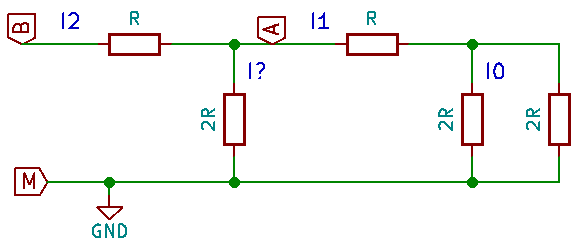
\includegraphics{images/TD/convAN_R2R_a.png}
\end{figure}


\begin{enumerate}
	\item Que vaut le courant $I_1$ en fonction du courant $I_0$ (courant passant par la résistance $2R$ ?

\answer{
On peut s'intéresser à la résistance équivalente entre les points A et M :

	On trouve entre A et M une résistance $R$ en série avec un ensemble en parallèle de 2 résistances de $2R$.
	
	$R_{AM} = R + (2R // 2R)$  avec $2R//2R = \frac{2R \cdot 2R}{2R + 2R} = R$
	
	On a alors : $R_{AM} = R + R = 2R$.

\medskip

Les deux résistances de $2R$ étant en parallèle, elles sont soumises à la même différence de potentiel. Comme elles ont également la même résistance, elles sont traversées par le même courant.

La loi des noeud au point d'intersection de $R$ et des deux résistances de $2R$ donne que $I_1 = 2 \cdot I_0$.
}	

	\item Que vaut le courant $I_2$ en fonction du courant $I_0$ (courant passant par la résistance $2R$ ?
	
\answer{
En reprenant le modèle équivalent du montage entre A et M, on obtient alors un nouveau montage R-2R.

On a alors $R_{BM} = R + (2R // 2R) = 2R$. Et ainsi de suite...

De la même façon que précédemment, on obtient $I_2 = 2 \cdot I_1 = 2^2 \cdot I_0$.
}		
	
\end{enumerate}

%%%%%%%%%%%%%%%%%%%%%%%%%%%%%%%%%%%%
\subsection*{Montage complet}

On s'intéresse à présent au montage suivant : 

\begin{figure}[!h]
	\centering
	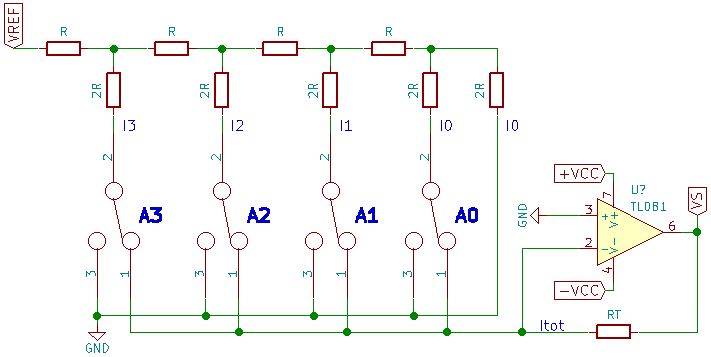
\includegraphics{images/TD/convAN_R2R_b.png}
\end{figure}

On supposera que lorsque $A_i = 0$, l'interrupteur $i$ est en position 3 et que lorsque $A_i = 1$, l'interrupteur $i$ est en position 1.

\begin{enumerate}
	\item Quel est le type de montage autour de l'ALI ?

\answer{Il s'agit d'un montage transimpédance, qui permet de transformer $I_{tot}$ en une tension $V_S = - R_T \cdot I_{tot}$.}

	\item En quoi la structure vue précédemment peut nous aider ?

\answer{
	On remarque que la structure est de type R-2R.
	En fonction de la position des $A_i$, le courant résultant des différentes branches va soit à la masse, soit dans le contre-réaction de l'ALI. Comme l'ALI est en mode linéaire, on a $V+ = V-$ et $V+ = 0$. Dans les deux cas, la masse est présente sur les interrupteurs $A_i$.
}

	\item Que vaut alors le courant $I_{tot}$ dans la contre-réaction de l'ALI en fonction des courants $I_i$ ?

\answer{
	Si on calcule le courant au noeud en $V-$, on a $I_{tot} = A_0 \cdot I_0 + A_1 \cdot I_1 + A_2 \cdot I_2 + A_3 \cdot I_3$.
	
	De manière généralisée : $I_{tot} = \sum_{k = 0}^{N} A_k\cdot I_k$
}	
	
	\item Que vaut alors le courant $I_{tot}$ dans la contre-réaction de l'ALI en fonction du courant $I0i$ et des valeurs des $A_i$ ?
	
\answer{
	D'après la section précédente, on a vu que $I_1 = 2^1 \cdot I_0$, que $I_2 = 2^2 \cdot I_0$...
	
	On a alors : $$I_{tot} = I_0 \cdot \sum_{k = 0}^{N} A_k\cdot 2^k$$
}
	
\end{enumerate}
